\documentclass[
	11pt, 
	DIV10,
	ngerman,
	a4paper, 
	oneside, 
	headings=normal, 
	captions=tableheading,
	final, 
	numbers=noenddot
]{scrartcl}


\usepackage[ruled]{algorithm2e}
\usepackage{graphicx}
\usepackage{hyperref}
\usepackage{amsmath}


\title{Fully Asynchronous SPH Simulation}
\subtitle{\vspace{0.5cm}Seminar: Current Topics in Fluid Animation}
\author{Yinglun Liu}


\begin{document}
\maketitle


\section{Motivation}

Over the years, the adoption of smoothed particle hydrodynamics(SPH) has developed to become the common pratice when simulating fluids in various scenes. In non-iterative approaches, the physical properties of a fluid particle is constantly influenced by its immediate neighborhood and is thereby updated in each time step following a procedure that helps compute the respective components in the Navier-Stokes equation. In these equations, the computation of new attributes of the current particle requires several times the access to information from its surrounding neighbors. Intuitively, a natural practice would be to, as did many non-iterative SPH solvers, perform global updates to all particles using a single uniform step size. While iterative SPH solvers nowadays generally yield better performances, traditional non-iterative approaches do not seem to lessen in popularity due to the fact that they are easy to implement and suitable for less turbulent fluids (see Fig. \ref{fig1}).

\begin{figure}[tb]
	\centering
	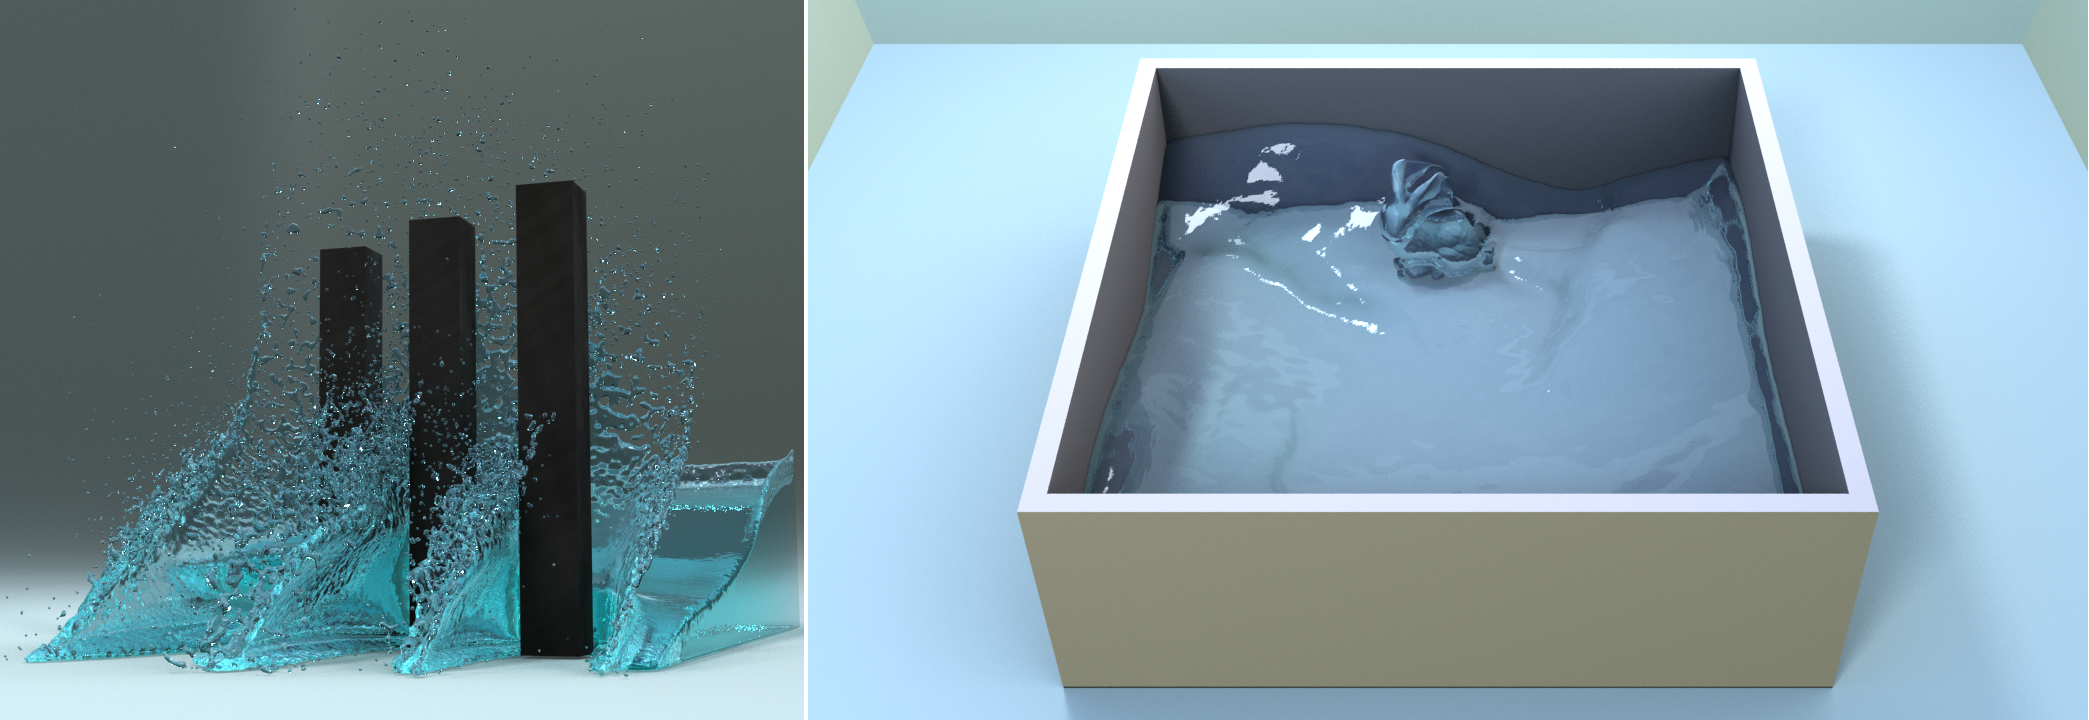
\includegraphics[scale=0.2]{images/3}
	\caption{\label{fig1} Animated scenes of dam break and radial flow demonstrate that non-iterative SPH solvers are capable of generating fluid scenes with high visual authenticity \cite{reinhardt2017fully}.
	}
\end{figure}

\par
Be that as it may, a core defect of non-iterative SPH solvers may lie in the lack of efficiency. On one hand, to enforce a constantly negligible density deviation within the fluid, large stiffness parameters are adopted to generate high pressures. Such selection of parameters demands smaller time steps and, in turn, a greater number of global iterations for stable and correct particle interations. This can lead to tremendously higher overhead for the generation of visually realistic animation, where tens of millions of particles are included to allow for as fine-grained details as possible. On the other hand, the paper made the observation that, while smaller time steps are essential in heavily interacting regions to guarantee stable simulation, in many less complex parts of the fluid the particles could do well with a larger time step (see Fig. \ref{fig2}). That is, the maximum possible step size for a particle varies substantially across different regions of the simulation, and it makes less sense to set one global step size for all particles, since it would inevitably be limited by the single particle with the strictest time constraint and lead to much waste of computational power. Previous works that attempted to tackle this aspect of the problem had to introduce some global synchronization barriers that improves consistency but somehow shadows the boost on performance due to waiting threads within parallel execution.

\begin{figure}[tb]
	\centering
	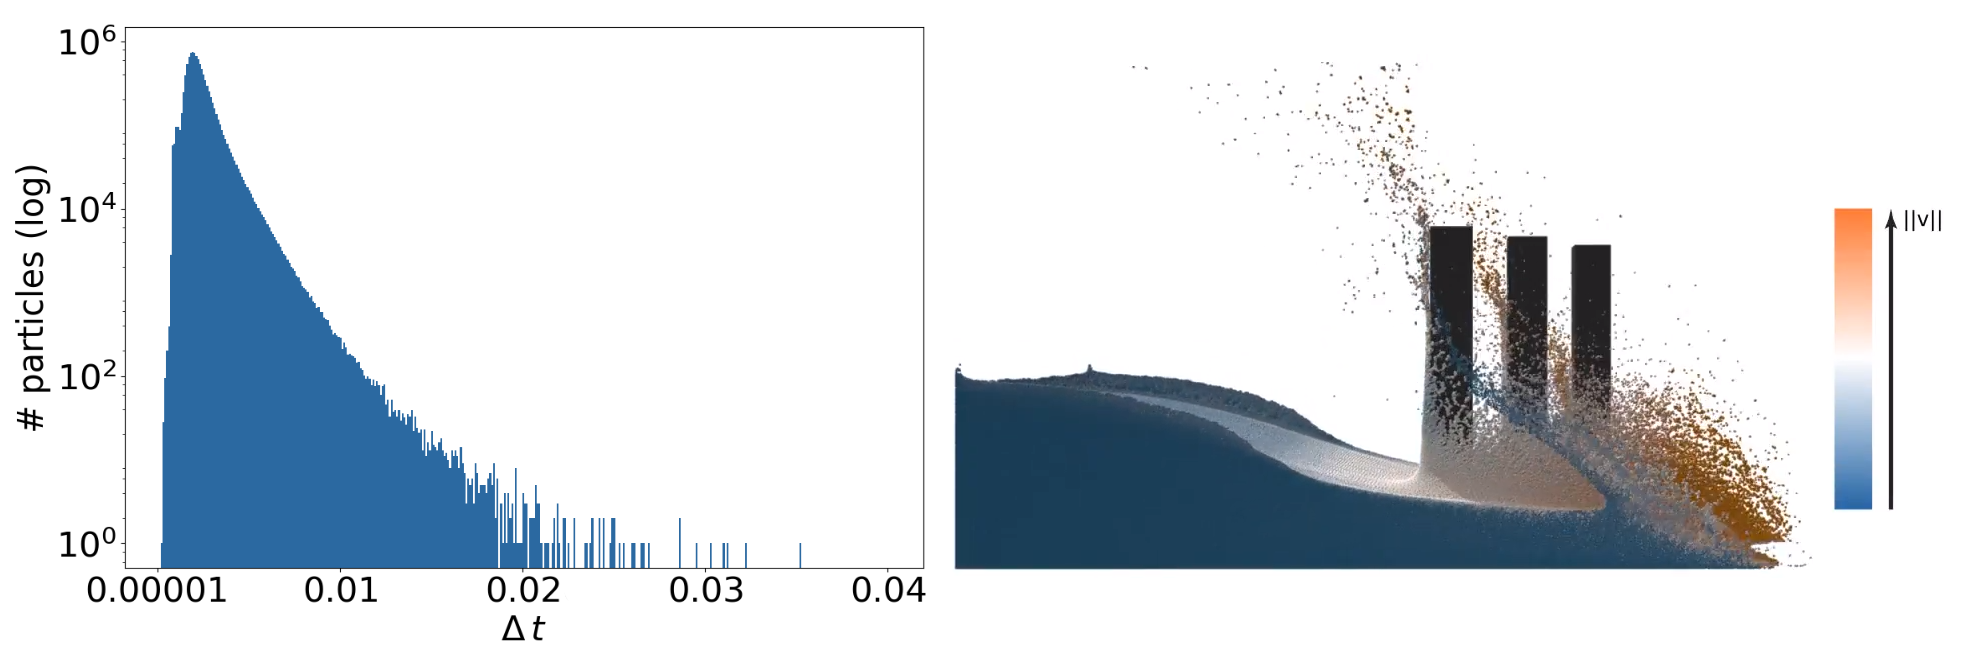
\includegraphics[scale=0.25]{images/1}
	\caption{\label{fig2} For fluid simulation based on SPH, the magnitude of velocity differs substantially across particles from different regions (right). As a result, the maximum possible step size for each individual particle could diverge to cover up to multiple magnitudes (left) \cite{reinhardt2017fully}.}
\end{figure}

\par
To cope with this, the paper proposes a novel method for the time integration of particles, in which each particle is assigned an individual step size and the whole simulation is carried out fully asynchronous. By handling each particle individually throughout the simulation, the solver expends less computational effort on smoother regions and considerably cut down the overall time consumption. To ensure consistency, the neighborhood is reconstructed at the current time stamp each time a particle is processed. To demonstrate the strength of the proposed method, the paper further proposes a multi-queue parallelization to such fully asynchronous integration procedure. Comparative experiments against related works were conducted under diverse conditions and environments to prove the efficacious enhancement on performance.

\section{Related Work}

Since the contribution of this paper focuses on the temporal adaptivity of SPH-based fluid simulations (i.e. how the step size of SPH integration models could be adapted to enhance the performance of the simulation) and how the proposed method could be parallelized, we discuss related works in these two directions separately.

\subsection{Temporal Adaptivity}

Extensive studies have been conducted on the temporal adaptivity of SPH models:

\begin{itemize}
    \item For synchronous SPH simulation, temporal adaptivity could be exploited as in \cite{desbrun1996smoothed}. For each global iteration the uniform step size is determined by the particle with the strictest CFL constraint. This scheme is also adopted by \cite{bender2010boundary}, who added an additional acceleration constraint as the second term to take into consideration the impact of large forces.
    \item \cite{goswami2014regional} introduces a regionally synchronous integration model. They divide all particles into separate regions depending on their maximum possible step size and fix a uniform step size for each region that is a multiple of the user-defined base value.
    \item \cite{desbrun1996smoothed} explored the possibility to apply individual times steps. For each particle the user-defined simulation step size is divided by powers of two to the extent such that the CFL condition is met. Forces are evaluated only at individual time steps to facilitate gains in performance. \cite{ban2018adaptively} follows this idea and proposes a semi-synchronous time stepping scheme. They introduce the concept of a virtual system time line that advances with the smallest individual step size of all particles. Particles with an individual step size that exceeds the gap between its own time stamp and the system checkpoint are deactivated and only propagated forward using linear interpolation. Those that are active are instead evaluated in the same procedure as in the fully synchronous setting. Such a stepping strategy still introduces a great number of global synchronization barriers although the overall operations are cut down to some extent.
\end{itemize}

\subsection{Parallelism in SPH Simulation}

Speeding up SPH simulations can also be achieved by exploiting parallelism:

\begin{itemize}
    \item For neighborhood search and access to particle properties, the community seems to have reached the consensus to utilize a uniform grid to facilitate concurrent queries of neighborhood information \cite{ihmsen2014sph}.
    \item For synchronous non-iterative SPH simulation, simple loop parallelization could be adopted, since several for-loops are responsible for computing the attributes of the particles in each global step.
    \item For \cite{goswami2014regional}, parallel computation should be straightforward to implement as for each region the step size is fixed. However, the solver could suffer from unbalanced load and the waiting threads since at the edge zones of the regions synchronization becomes inevitable.
    \item For \cite{ban2018adaptively}, since in each global synchronization barrier the solver performs either full integration or linear interpolation on all particles, the parallelization scheme bears little difference to the fully synchronous setting.
\end{itemize}

\section{Non-iterative SPH}

Governed by the Navier-Stokes equation \eqref{eq1}, non-iterative SPH performs interpolation over the neighborhood of a particle to calculate its attributes and ultimately the forces it incurs within one time step of the simulation. The fluid attribute $ A_{i} $ of particle i at position $ \boldsymbol{x}_{i} $ is computed as the weighted sum of  $ A_{j} $ over all neighboring particles j, with the weights given by a user-defined kernel function W that satisfies the following conditions:

\begin{itemize}
    \item The function has an integral value of one over its acting domain.
    \item The function approximates the $ Dirac $-$ \delta $ distribution as its smoothing length approaches zero.
    \item The function is non-negative.
    \item The function is symmetric.
    \item The function is of compact support (i.e. the function value remains zero beyond its smoothing length).
\end{itemize}

After all forces are computed, time integration methods like symplectic Euler or leap frog is carried out to update particle position and speed. Denoting with $p$ the pressure, $\boldsymbol{v}$ the velocity and $\rho$ the density of a particle, a typical formulation of the Navier-Stokes equation models the acceleration of a particle as

\begin{equation}
	\label{eq1}
	\frac{\delta \boldsymbol{v}}{\delta t} = -\frac{\nabla p}{\rho} + \nu \nabla^{2} \boldsymbol{v} + \frac{\boldsymbol{F}^{external}}{\rho},
\end{equation}

where $ \nu $ is the kinematic viscocity of the liquid and the three terms on the right hand side of the equation describes per unit volume the impact of pressure forces, viscosity forces and external forces respectively. 

\subsection{SPH Procedure with splitting}

The paper adopts here the splitting strategy as described by \cite{ihmsen2014sph}, where for each update step the advection forces $ \boldsymbol{F}^{advection} $ are separately computed and then used to calculate an intermediate advection velocity $ \boldsymbol{v}^{*} $. An advection density $ \rho^{*} $ is introduced to represent the expected density at the end of this time step as a result of the divergence in the velocity field assuming no compensating pressure force is generated. pressures $ p $ and pressure forces $ \boldsymbol{F}^{pressure} $ are afterwards handled conventionally. This updating scheme forces the solver to implicitly consider the impact of advection forces before generating pressure forces to counteract the deviation of density and therefore stablizes the simulation.
\par
Conventionally, a single global update step with the concept of spitting applied proceeds as in Alg. \ref{alg1}. To interpolate particle properties a neighborhood search is conducted at each time step to fetch the set of neighbors for each particle. Since such operations can be computationally expensive, spatial data
structures(e.g. a uniform grid) that supports parallel operations are usually constructed at the beginning to accelerate the process. At each global step, the grid cells are queried and updated to efficiently maintain neighborhood information. To further minimize time consumed by inevitable query operations at each time step, particles are sorted in accordance with their spatial cell. In this way, spatially adjacent particles are stored on adjacent memory slots, enhancing the cache-hit rates during the simulation. Here, the paper chooses Z-order curve (see Fig. \ref{fig6}), a commonly used sorting function that effectively preserves spatial locality due to its fractal block structure, for particle indexing.

\begin{figure}[tb]
	\centering
	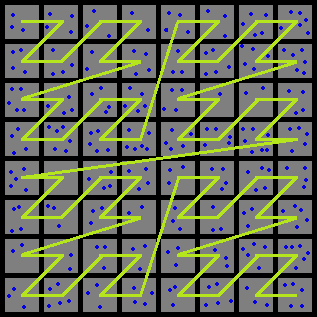
\includegraphics[scale=0.5]{images/z}
	\caption{\label{fig6} A Z-order curve in 2-dimensional space.}
\end{figure}

\large
\begin{algorithm}
	\DontPrintSemicolon
	\SetAlgoLined
	\SetAlgorithmName{Algorithm}{Algorithm}{List of Algorithms}
	\SetAlCapNameFnt{\large}
	\SetAlCapFnt{\large}
	\caption{\label{alg1} One global step with splitting \cite{reinhardt2017fully}}
	\SetKwFunction{FMain}{GlobalStep}
	\SetKwProg{Fn}{Function}{:}{}
	\Fn{\FMain{}}{
		\For{each particle i}{
			find neighbors j\;
		}
		\For{each particle i}{
			compute advection force $ \boldsymbol{F}_{i}^{*} = \boldsymbol{F}_{i}^{viscosity} + \boldsymbol{F}_{i}^{ext} $\;
			compute advection velocity $ \boldsymbol{v}_{i}^{*} $ using $ \boldsymbol{F}_{i}^{*} $\;
		}
		\For{each particle i}{
			compute advection density $ \rho_{i}^{*} $\;
			compute pressure $ p_{i} $\;
		}
		\For{each particle i}{
			compute pressure force $ \boldsymbol{F}_{i}^{*} $\;
			compute new particle velocity $ \boldsymbol{v}_{i}(t + \delta t) $\;
			compute new particle position $ \boldsymbol{x}_{i}(t + \delta t) $\;
		}
	}
\end{algorithm}
\normalsize

The advection force incurred by a particle consists of a viscosity component and some external components. Viscosity forces counteract divergence of the velocity field and is hence proportional to the second-order spatial derivative of velocity. But since second-order derivatives are tricky to compute, the approximation form proposed originally by \cite{monaghan1992smoothed} is prefered instead. Therefore the viscosity component acting on particle i is computed as

\begin{equation}
	\label{eq2}
	\boldsymbol{F}_{i}^{viscosity} = 2m_{i}\nu \sum_{j}\frac{m_{j}}{\rho_{j}}\boldsymbol{v}_{ij}\frac{\boldsymbol{x}_{ij} \cdot \nabla W_{ij}}{\boldsymbol{x}_{ij}\cdot \boldsymbol{x}_{ij} + 0.01h^{2}},
\end{equation}

where $m_{i}$ denotes the mass of particle i, $\boldsymbol{v}_{ij} = \boldsymbol{v}_{i} - \boldsymbol{v}_{j}$ and $\boldsymbol{x}_{ij} = \boldsymbol{x}_{i} - \boldsymbol{x}_{j}$. Since modeling boundary interations and surface tension is not a core theme of this paper, the paper directly adopts the method of \cite{akinci2012versatile} and \cite{huber2015evaluation} to handle these two aspects of the advection force.
\par
Based on the advection forces, intermediate advection velocity is computed as

\begin{equation}
	\label{eq3}
	\boldsymbol{v}_{i}^{*} = \boldsymbol{v}_{i}(t) + \delta t_{i}\frac{\boldsymbol{F}_{i}^{advection}}{m_{i}}.
\end{equation}

This equation can be perceived as an intermediate velocity update using symplectic Euler without considering the impact of pressure forces. The first-order spatial derivative of velocity reflects the divergence of the velocity field and is used to compute the advection density. Again, the paper chooses the robust variant presented by \cite{monaghan1992smoothed} and computes the advection density via

\begin{equation}
	\label{eq4}
	\rho_{i}^{*} = \sum_{j}m_{j}W_{ij} + \delta t_{i}\sum_{j}(\boldsymbol{v}_{i}^{*} - \boldsymbol{v}_{j}^{*})\cdot \nabla W_{ij},
\end{equation}

where the first term describes the static density at particle position $ \boldsymbol{x}_{i} $ and the second term describes the density change during step $ \delta t_{i} $ as a consequence of diverging velocity field.
\par
Having obtained the advection densities of the particles, pressure at particle position $ \boldsymbol{x}_{i} $ is computed as

\begin{equation}
	\label{eq8}
	p_{i} = k(\rho_{i}^{*} - \rho_{0}),
\end{equation}

where $ \rho_{0} $ is the system's reference density and k is the stiffness parameter. Negative pressures are clamped to zero as in \cite{ihmsen2013implicit} to prevent the water splashes from being absorbed as a result of the induced cohesive effect. Finally, the respective pressure forces are calculated using the momentum-preserving variant:

\begin{equation}
	\label{eq5}
	\boldsymbol{F}_{i}^{pressure} = -m_{i}\sum_{j}m_{j}\left(\frac{p_{i}}{(\rho_{i}^{*})^{2}} + \frac{p_{j}}{(\rho_{j}^{*})^{2}}\right)\nabla W_{ij}.
\end{equation}

This pressure force is then solely responsible for the explicit velocity and position update of the particle, which we discuss in the next subsection.

\subsection{Time Integration}

Despite the fact that multiple common numerical time integration schemes would fit well into the framework of non-iterative SPH solvers, the paper employs a modified version of symplectic Euler:

\begin{equation}
\begin{split}
	\label{eq6}
	\boldsymbol{v}_{i}(t_{i} + \delta t_{i}) &= \boldsymbol{v}_{i}(t_{i}) + \delta t_{i}\frac{\boldsymbol{F}_{i}^{pressure}(t_{i})}{m_{i}} \\
	\boldsymbol{x}_{i}(t_{i} + \delta t_{i}) &= \boldsymbol{x}_{i}(t_{i}) + \delta t_{i}\boldsymbol{v}_{i}(t_{i} + \delta t_{i}) + \frac{\delta t_{i}^{2}}{2}\frac{\boldsymbol{F}_{i}^{pressure}(t_{i})}{m_{i}}.
\end{split}
\end{equation}

In addition to a first-order Taylor expansion, a second-order term is added here to the position updating equation to facilitate stabler behavior when applying larger time steps. For numerical stability and correct behavior of the particles, the size of each global time step has to be chosen in a way such that it fulfills the CFL condition. Intuitively, CFL condition enforces that a particle does not travel in one time step a distance that exceeds the smoothing length of the interpolating kernel, which is typically set to be twice as large as the initial particle spacing $r_{i}$. Such a constraint could guarantee that a particle does not leap over its spatial neighbors and thus fail to interact properly with them. Similarly, \cite{bender2010boundary} introduces a constraint on acceleration of the particle that targets the same outcome. Putting these two constraints together, the maximum step size for an individual particle is given by:

\begin{equation}
	\label{eq7}
	\delta t_{i} = min(\lambda_{v}\frac{2r_{i}}{|\boldsymbol{v}_{i}|}, \lambda_{F}\sqrt{\frac{2r_{i}}{\boldsymbol{F}_{i}^{pressure}/m_{i}}}),
\end{equation}

where $ \lambda_{v} $ and $ \lambda_{F} $ scales the two terms respectively. In previous approaches where a globally adaptive stepping scheme is used, the system-wide step size is naturally chosen to be minimum of Eq. \eqref{eq7} over all particles.


\section{Fully Asynchronous SPH}

As explained in previous sections, conventional approaches of fixed or globally adaptive time stepping squander computational resources on particles that could have been integrated with larger time steps. Former works that try to mitigate the waste on computational power suffer from waiting threads since they introduce multiple times more synchronization barriers within the duration of the simulation. Therefore, the paper proposes to assign to each individual particle a dedicated step size determined by Eq. \eqref{eq7} and avoid any global synchronization barrier. Only a virtual export barrier is employed from time to time to fetch particle states for rendering purposes. A comparative illustration of the proposed method is given in Fig. \ref{fig3}.

\subsection{Sequential Execution of Asynchronous Simulation}

To achieve such asynchronous SPH simulation, the solver has to constantly ensure that the current particle $ i $ has immediate access to the attributes of its neighboring particles at time stamp $ t_{i} $. Since all particles advance through time independently, this can only be achieved if the attribute $ A_{j} $ of any neighbor $ j $ can be temporally interpolated as

\begin{equation}
	\label{eq9}
	\delta A_{j}(t_{i}) = A_{j}(t_{j}) + (t_{i} - t_{j})\frac{\delta A_{j}(t_{j})}{\delta t}.
\end{equation}

Fortunately, by employing the splitting concept, the non-iterative SPH integration already provides a feasible way to conduct such reconstruction efficiently.

\begin{figure}[tb]
	\centering
	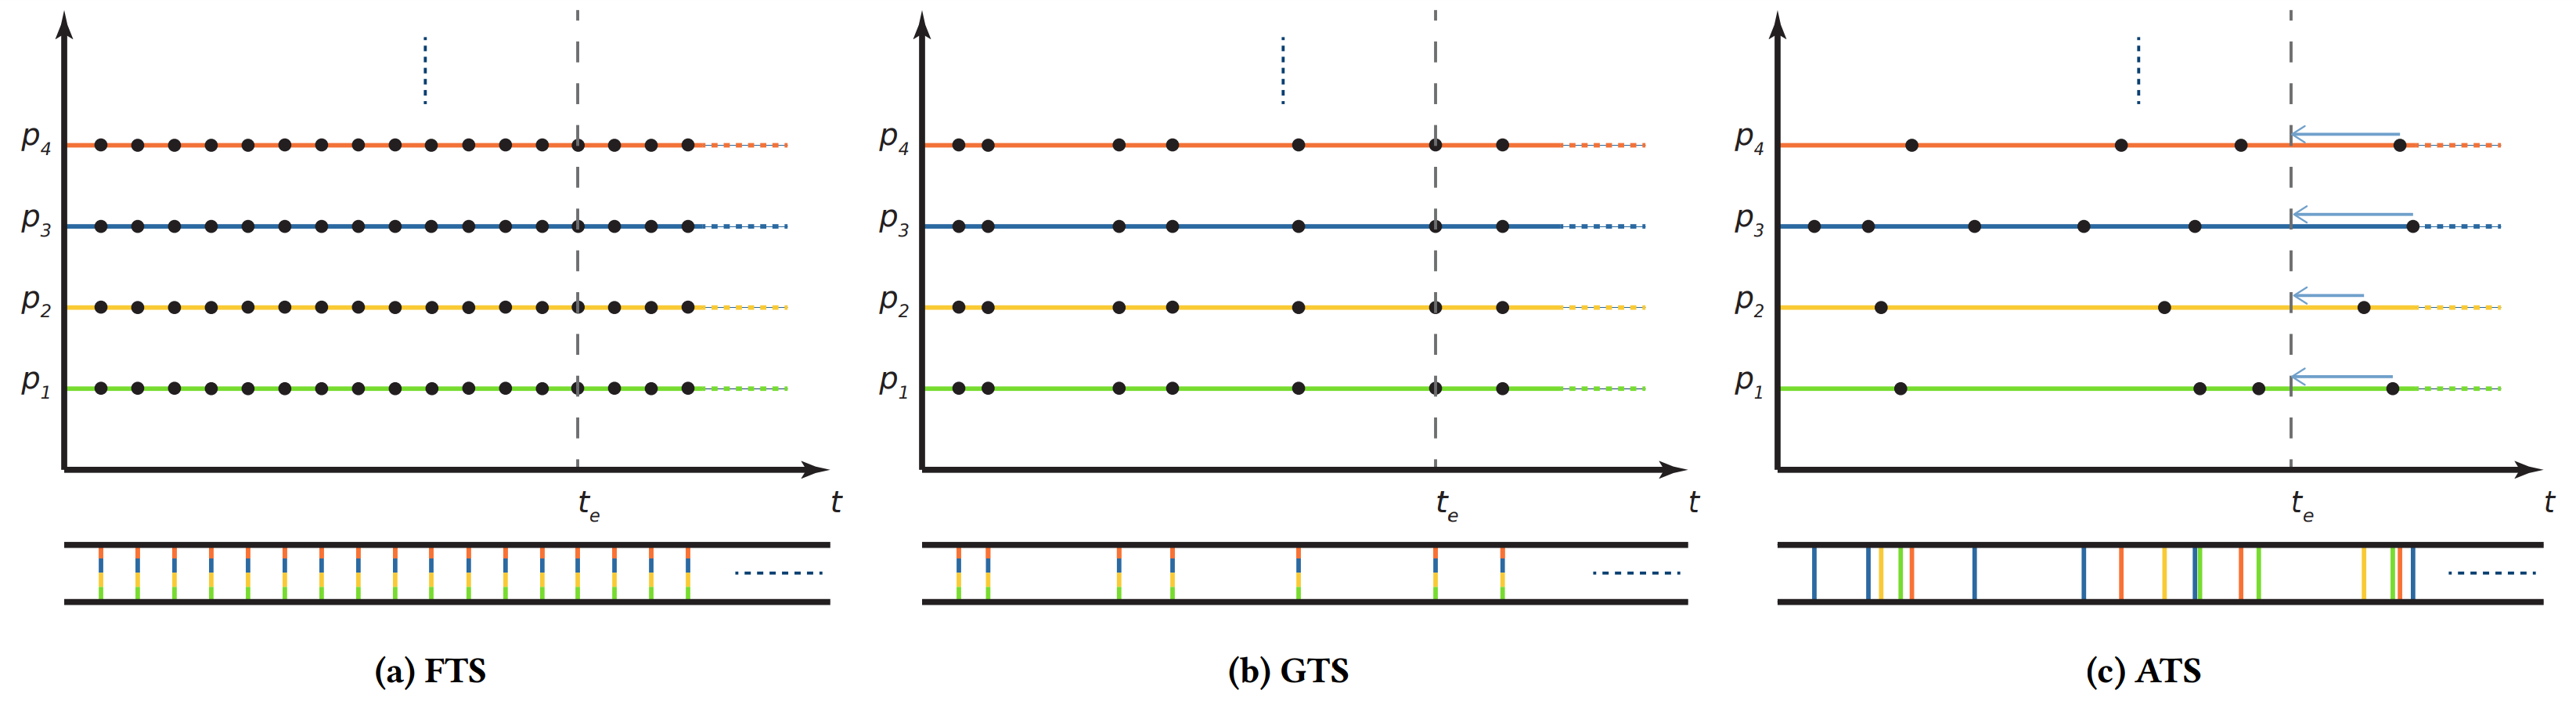
\includegraphics[scale=0.16]{images/4}
	\caption{\label{fig3} Illustration of various time stepping methods: (a) fixed time stepping (FTS), (b) globally adaptive time stepping (GTS), and (c) asynchronous time stepping (ATS). Note that with FTS and GTS all particles are updated simultaneously at each time step. With ATS each particle freely advances in time at its own pace, minimizing the overall computational expenditure. Only virtual barriers are need for exporting the outcome of the simulation. A priority queue is required to enforce a strict particle processing order for attribute consistency. \cite{reinhardt2017fully}.}
\end{figure}

\par
Similar to Alg. \ref{alg1}, one step of integration for an individual particle has the following dependencies:

\begin{itemize}
    \item The viscosity force $ \boldsymbol{F}_{i}^{viscosity}(t_{i}) $ incurred by particle $i$ is dependent on the positions $ \boldsymbol{x}_{j}(t_{i}) $ and velocities $ \boldsymbol{v}_{j}(t_{i}) $ of neighboring particles $j$.
    \item The advection density $ \rho_{i}^{*} $ of particle $i$ is dependent on the advection velocities $ \boldsymbol{v}_{j}^{*} $ of neighboring particles $j$.
    \item The pressure force $ \boldsymbol{F}_{i}^{pressure}(t_{i}) $ incurred by particle $i$ is dependent on the advection densities $ \rho_{j}^{*} $ and pressures $ p_{j} $ of neighboring particles $j$.
\end{itemize}

Since velocity and position can be directly pushed forth or back in time under the symplectic Euler scheme, velocities $ \boldsymbol{v}_{j} $ and positions $ \boldsymbol{x}_{j} $ of neighboring particles $j$ are reconstructed at the current time stamp $ t_{i} $ to facilitate computation of viscosity force of the current particle. Since the second term in Eq. \eqref{eq4} approximates the temporal derivative of density, advection densities $ \rho_{j}^{*} $ of neighboring particles $j$ can be direcly pushed forth or back in time to facilitate computation of pressure force. The pressure $ p_{j} $ of neighboring particles at the current time stamp $ t_{i} $ can be computed as usual since they do not induce a high expense. Since the reconstruction of the advection velocities $ \boldsymbol{v}_{j}^{*} $ of neighboring particles could be costly, we may assume that the paper replaces $ \boldsymbol{v}_{j}^{*}(t_{i}) $ with $ \boldsymbol{v}_{j}(t_{i}) $ to cut down the total amount of operations for neighborhood reconstruction in a single particle state update. Alg. \ref{alg2} describes the outline of one individual simulation step. An illustration of the neighborhood reconstruction scheme is given in Fig. \ref{fig4}.

\large
\begin{algorithm}
	\DontPrintSemicolon
	\SetAlgoLined
	\SetKwFunction{FMain}{IndividualStep}
	\SetAlgorithmName{Algorithm}{Algorithm}{List of Algorithms}
	\SetAlCapNameFnt{\large}
	\SetAlCapFnt{\large}
	\caption{\label{alg2} One individual step in ATS \cite{reinhardt2017fully}}
	\SetKwProg{Fn}{Function}{:}{}
	\Fn{\FMain{particle $i$}}{
		determine maximum possible step size $ \delta t_{i} $\;
		\;
		reconstruct velocities $ \boldsymbol{v}_{j}(t_{i}) $ and positions $ \boldsymbol{x}_{j}(t_{i}) $ of neighbors $j$ at $t_{i}$\;
		\;
		compute viscosity force $ \boldsymbol{F}_{i}^{viscosity}(t_{i}) $ incurred by particle $i$ using Eq. \eqref{eq2}\;
		compute external forces $ \boldsymbol{F}_{i}^{ext}(t_{i}) $ incurred by particle $i$\;
		compute advection force $ \boldsymbol{F}_{i}^{*}(t_{i}) $ incurred by particle $i$\;
		compute advection velocity $ \boldsymbol{v}_{i}^{*}(t_{i}) $ of particle $i$ using Eq. \eqref{eq3}\;
		compute advection density $ \rho_{i}^{*} $ of particle $i$ using Eq. \eqref{eq4}\;
		compute pressure $ p_{i} $ of particle $i$ using Eq. \eqref{eq8}\;
		\;
		reconstruct advection densities $ \rho_{j}^{*} $ and pressures $ p_{j} $ of neighbors $j$ at $t_{i}$\;
		\;
		compute pressure force $ \boldsymbol{F}_{i}^{pressure}(t_{i}) $ incurred by particle $i$ using Eq. \eqref{eq5}\;
		\;
		integrate particle $i$ over time using $ \delta t_{i} $\;
	}
\end{algorithm}
\normalsize

\begin{figure}[tb]
	\centering
	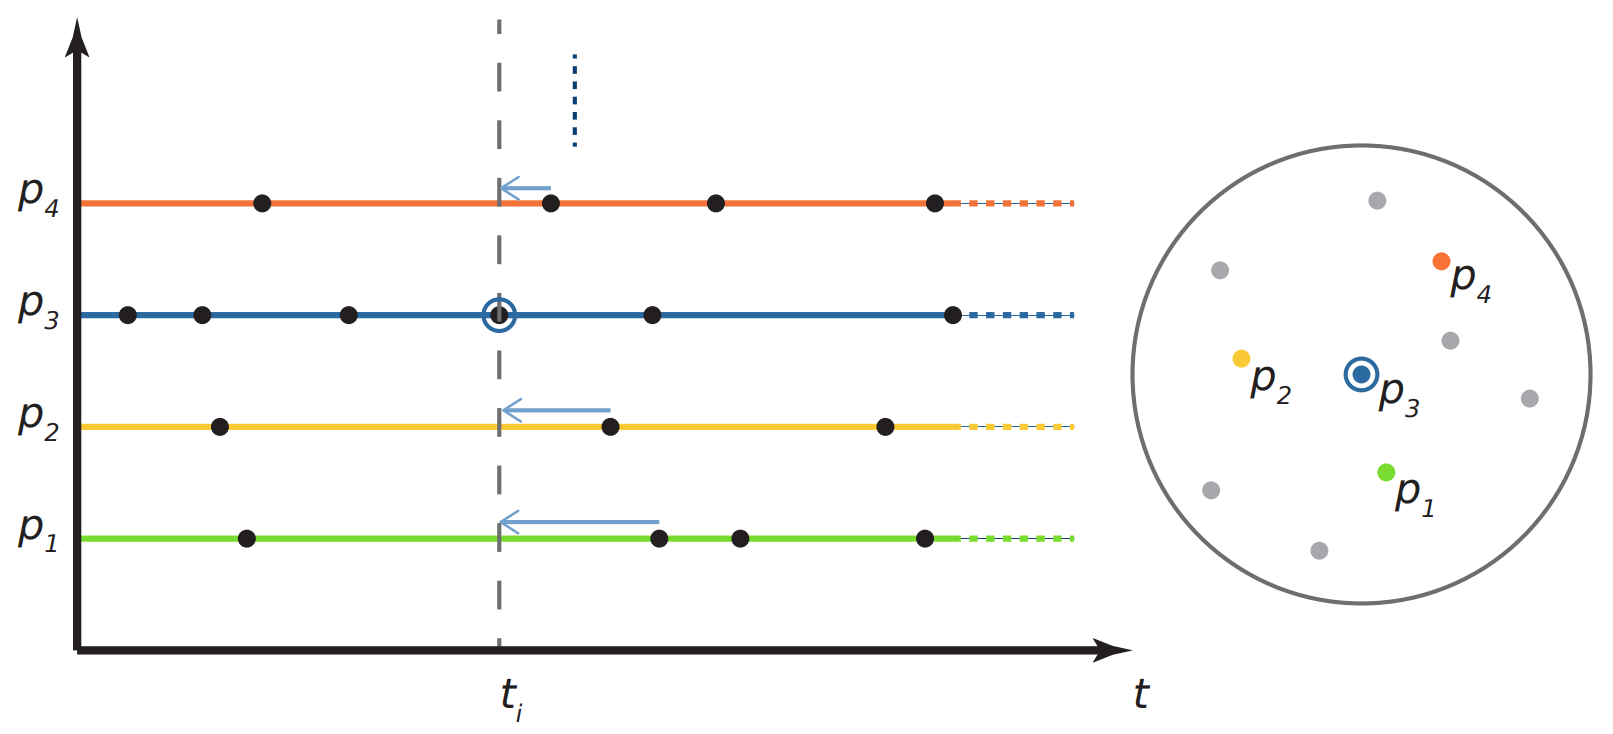
\includegraphics[scale=0.25]{images/5}
	\caption{\label{fig4} Illustration of the neighborhood reconstruction scheme: attributes of neighbors of particle $p_{3}$ are traced back in time to support the computations at the current time step. A particle is processed only when all its neighbors are already temporally ahead of itself. In this particular scenario particle $ p_{4} $ reaches the head of the priority queue after particle $p_{3}$ finishes its individual step \cite{reinhardt2017fully}.}
\end{figure}

To guarantee stable and correct behavior of the algorithm, the paper stipulates empirically that the attributes of neighboring particles should only be traced back in time. In other words, a particle is only to be processed if its entire neighborhood is more advanced in time than itself. To explicitly enforce such strict processing order, a priority queue storing only particle indices is introduced to constantly arange the particles in chronological order. Specificaly, until the next virtual export barrier is reached, the solver repeatedly dequeues the particle at the top of queue, performs one individual step for the particle and then inserts its index back into the queue such that the chronological order within the queue is sustained. After the last particle reaches the next virtual export barrier $t_{exp}$, the attributes of all particles that are demanded by the rendering process are reconstructed at $t_{exp}$ using the same procedure as stated above.

\subsection{Parallelization}

A parallel implementation of the aforementioned time stepping scheme is not straightforward given the restriction on processing order. Naively spawning multiple queues and handling them independently would lead to violation of the ordinal constraint. Adopting simple synchronization strategies could cause multiple threads to be stuck at each other when several particles have neighbors in other queues that lag behind in time, which could force their belonging queues to hang up until the ordinal constraint is fulfilled. To cope with this undesirably inherent character of the devised approach, the paper introduces per queue a waiting list as the buffer area. When the solver of a queue runs into a particle that violates the ordinal constraint, this particle is removed and pushed into the waiting list (see Fig. \ref{fig5}). The solver then goes on to process the particle at the top of the queue until a predefined interval is reached and all particles in the waiting list are reinserted into the queue. Alg. \ref{alg3} describes the running process of a priority queue.

\begin{figure}[tb]
	\centering
	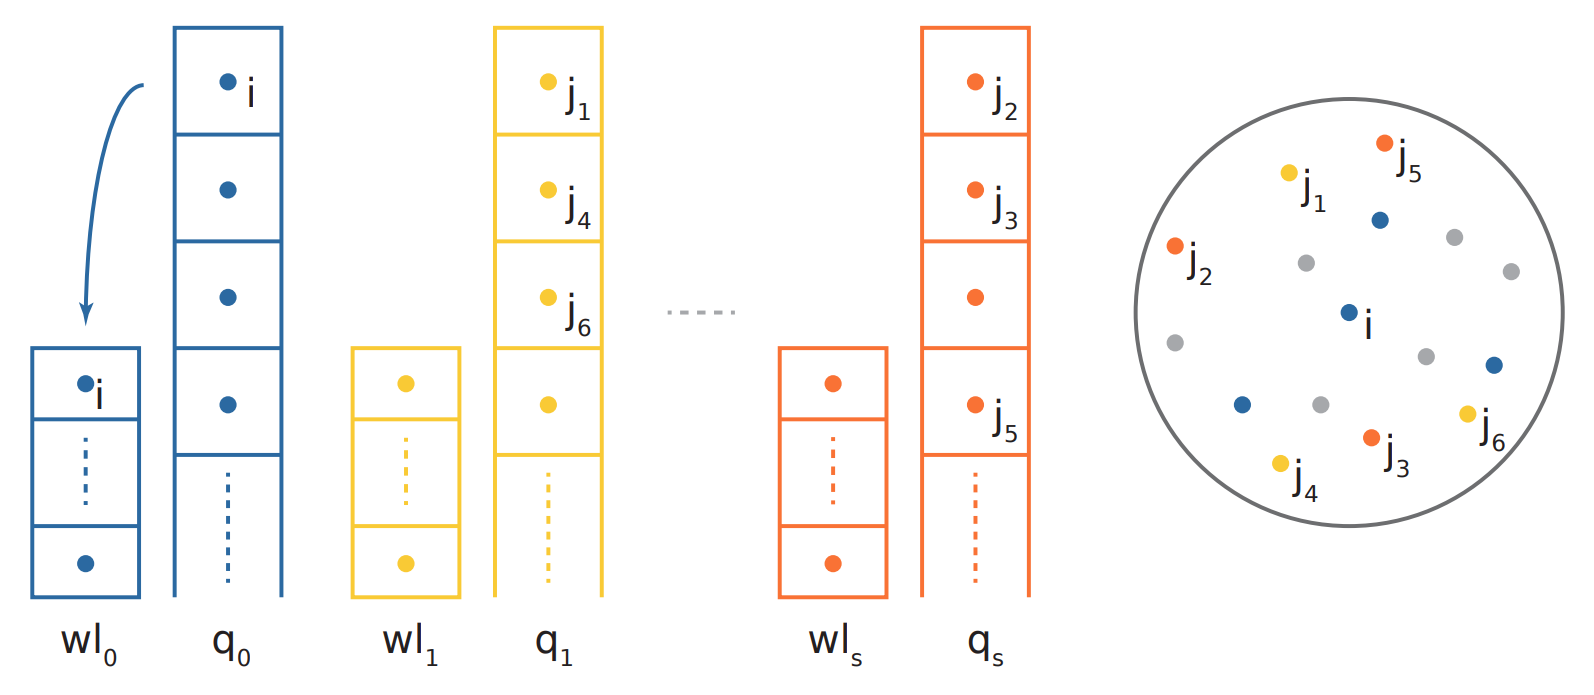
\includegraphics[scale=0.25]{images/6}
	\caption{\label{fig5} Illustration of the waiting list: the strict particle processing order could be violated when using multiple queues for parallel computation. If a particle at the head of queue $ q_{0} $ has a neighbor in another queue that is less advanced in time, the solver moves it from $ q_{0} $ and stores it on the accompanying waiting list $ wl_{0} $ \cite{reinhardt2017fully}.}
\end{figure}

\large
\begin{algorithm}
	\DontPrintSemicolon
	\SetAlgoLined
	\SetAlgorithmName{Algorithm}{Algorithm}{List of Algorithms}
	\SetAlCapNameFnt{\large}
	\SetAlCapFnt{\large}
	\caption{\label{alg3} Running process of a priority queue \cite{reinhardt2017fully}}
	\SetKwFunction{FMain}{RunQueue}
	\SetKwProg{Fn}{Function}{:}{}
	\Fn{\FMain{queue $q$, time stamp $ t_{exp} $}}{
		Initialize waiting list $ wl $\;
		Initialize step count $ cnt $\;
		\While{$ t_{q.top()} <  t_{exp} $}{
			$i$ = q.pop()\;
			find all neighbors $j$ of particle $i$\;
			\uIf{$ t_{i} < t_{j} $ for all neighbors $j$ of particle $i$}{
				IndividualStep(i)\;
				$ t_{i} = \delta t_{i} + 1$\;
				compute $ \delta t_{i} $ for next iteration\;
				q.push(i)\;
			}
			\Else{
				wl.push(i)\;
			}
			$ cnt = cnt + 1 $\;
			\uIf{cnt == INTERVAL}{
				insert all particles k in wl into queue\;
				empty wl\;
			}
		}
	}
\end{algorithm}
\normalsize

The proposed parallelization scheme presupposes a few conditions to ensure its efficiency. To justify the feasibility of the approach, we need to investigate a few implementation details with discretion.

\paragraph{Step size clipping}
Despite global synchronization barriers are avoided throughout the simulation, in practice it still helps to clip the individual time steps to be a multiple of 0.5 ms as in \cite{goswami2014regional}: Chances are high that spatially adjacent particles tend to be assigned the same step size. When a particle has a neighbor that is equally advanced in time thanks to this clipping operation, the reconstruction of this particular neighbor could be omitted. This could be a huge drop in amount operations for interaction-intensive regions.

\paragraph{Maintenance of neighborhood information}
To grant efficient query and update of particle neighbors, a uniform grid storing the cells in a one-dimensional array using Z-curve indexing is employed. Since the full construction of such spatial data structure induces a high computational expenditure, a global update of all grid cells is only carried out at each virtual export barrier. To ensure the correctness of a usual neighborhood search implementation, the particles have to be monitored each time they advance in space and time. If a particle changes cell after one individual step, a reference to the particle is instantly added to the new cell without removing the old reference. This is to deal with cases where one neighbor $j$ of a particle $i$ is no longer in $i$'s vicinity after advancing but by the current time stamp $t_{i}$ it still was and should contribute to particle $i$'s attribute computation. Since the kernel function is of compact support, such cell update strategy does not lead to false neighbors and only induces a small extra cost.

\paragraph{Queue splitting}
Since a Z-curve indexing of the particle arrays is employed, spatially close particles are assigned to the same queues by simply splitting the queues by particle index. Such property is desirable in the sense that if a particle has too many neighbors that appear in other queues it would inevitably be frequently put into the waiting list. Nevertheless as particles travel during the simulation, such spatial separation is detrimented. The paper proposes to reinitialize the queues after several virtual export barriers to improve spatial clustering among the particles. Empirically, a reinitialization of the queues is done every half of a second, which serves as a good trade-off between the overhead of reconstructing queues and postponing too many particles that violate the strict particle processing order.

\paragraph{Waiting list handling}
Detemining the interval to reinsert the postponed particles back into the queue is of vital significance. An interval too small would lead to postponing these violating particles multiple times while a restoration too late would mean to postpone their neighbors in other queues and result in threads stuck at each other. An optimal choice of this hyperparameter relies heavily on the complexity of the scene and is hence done empirically.

\section{Experiments}
In this section, comparative experiments against previous methods including fixed time stepping (FTS), globally adaptive time stepping (GTS) \cite{desbrun1996smoothed} and individual stepping (ITS) \cite{ban2018adaptively} are conducted to demonstrate the boost on performance for the proposed method. Particles are rendered as spheres for visual comparison to avoid losing details in surface. The methods of \cite{reinhardt2017visual} and \cite{bhatacharya2011level} are adopted for sphere and surface rendering respectively.

\subsection{Performance Study}
To focus on high performance, the largest possible step size that still maintains a stable simulation is used in all scenarios. Serial execution of all four methods are tested on two Corner-Dam-Break (CDB) scenes with 27k particles (in a cube of 30 x 30 x 30) and 125k particles (in a cube of 50 x 50 x 50) respectively. For parallel execution, three additional larger scenes are included to fully demonstrate the performance and scalability of the methods:

\begin{itemize}
    \item A Radial-Flow (RF) scene. This scene features a radial force field that, serving as an external force, drives the fluid particles and generates a vortex flow. A rigid body is placed in the fluid to disturb the flow. The whole scenario consists of 300k fluid and 20k boundary particles.
    \item A Fountain (FN) scene. This scene features a linear force field that propels the fluid particles upwards to generate a fountain. Upon falling down, the particles collide with a slightly deformed cone to form a non-symmetric flow. The whole scenario consists of 1.3M fluid and 16k boundary particles.
    \item A Dam-Break (DB) scene. This scene features three collision cylinders that induces strong impact for the fluid particles. 10M particles constitute the whole scenario.
\end{itemize}

\begin{table}[tb]
	\centering
	\begin{tabular}{|r|r|r|r|r|r|r|}
		\hline
		threads & scene & particles & FTS & GTS & ITS & ATS \\
		\hline
		& & & runtime & speedup & speedup & speedup \\
		\hline	
		1 & CDB & 27k & 396.9 & 3.0 & 4.4 & 7.5 \\
		1 & CDB & 125k & 1896.7 & 2.5 & 3.6 & 7.3 \\
		6 & CDB & 27k & 87.17 & 2.8 & 4.1 & 6.3 \\
		6 & CDB & 125k & 375.9 & 2.2 & 3.2 & 6.8 \\
		6 & RF & 300k & 926.7 & 1.3 & 3.0 & 7.5 \\
		6 & FN & 1.3M & 3245.6 & 1.7 & 2.3 & 4.4 \\
		6 & DB & 10M & 25973.0 & 1.8 & - & 6.3 \\
		\hline
	\end{tabular}
	\caption{\label{tab1} Performance comparison on various scenarios \cite{reinhardt2017fully}. Runtimes are measured in seconds.}
\end{table}

Tab. \ref{tab1} exhibits the runtime and speedup factor of all four stepping methods under different scenerios. Judging from the outcome of the experiments, ATS outperforms all the other methods using either serial or parallel execution while maintaining a stable and realistic silmulation (see Fig. \ref{fig7}). It can be observed that the speedup factor increases as expected when the scale of the scene is enlarged. This is mainly due to the fact that the additional workload induced by handling the waiting list tend to be less influential compared to the overall computational cost when larger amount of particles are included. There is however one thing worth noting: Despite ATS still yields the best performance in the Fountain scenario, the speedup factor turns out to be less impressive than other scenes. The paper attributes the decline in performance to a lack of interation in the scene: As the fountain scenario contains a large amount of almost static particles, the speedup gained with individual time steps becomes less decisive.

\begin{figure}[tb]
	\centering
	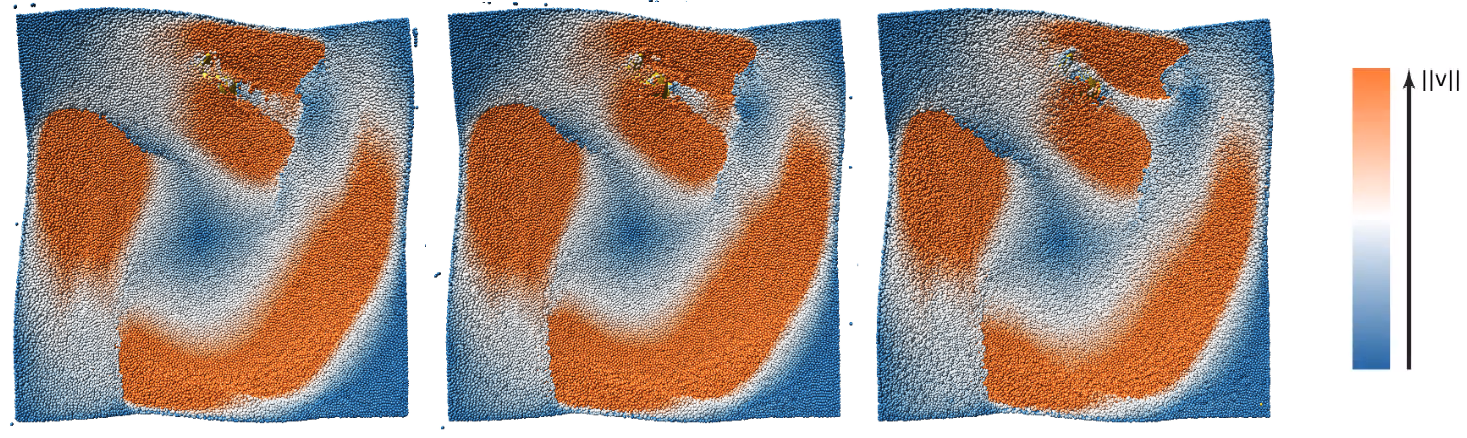
\includegraphics[scale=0.26]{images/2}
	\caption{\label{fig7} Visual comparison on the magnitude of particle velocities in Radial-Flow scene\cite{reinhardt2017fully}. From left to right are the velocity fields generated by GTS, ITS and ATS respectively. Only negligible difference could be identified in the flow pattern behind the collision object.}
\end{figure}

\begin{figure}[tb]
	\centering
	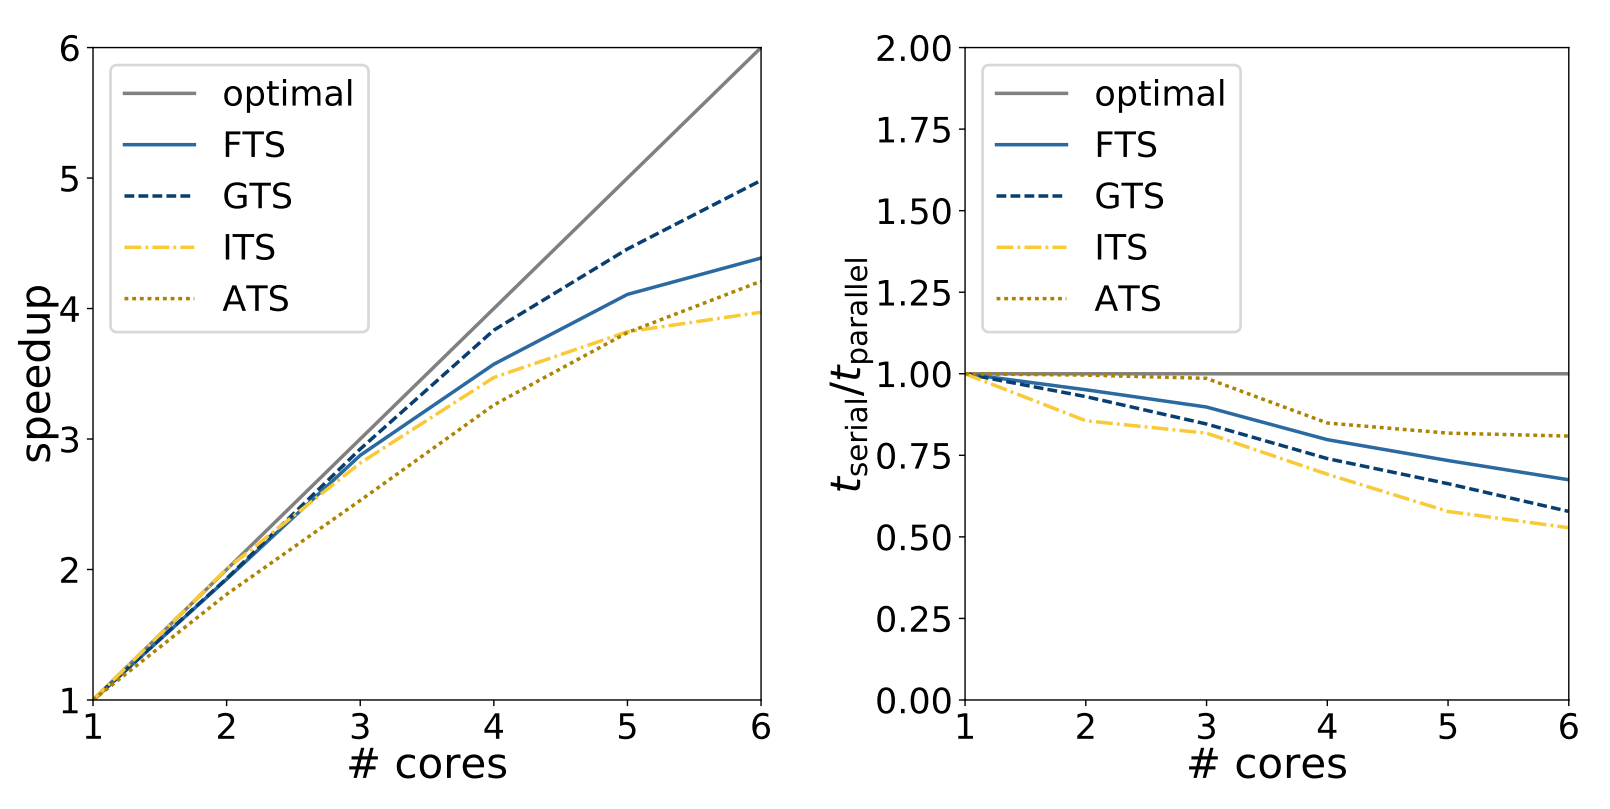
\includegraphics[scale=0.2]{images/8}
	\caption{\label{fig8} Visual comparison on the scalability of different time stepping models \cite{reinhardt2017fully}. The strong scaling performance of ATS seems to be less than satisfactory thanks to its extra effort spent on queue and waiting list handling. Nevertheless, in weak scaling test it significantly outperforms all other approaches.}
\end{figure}

\subsection{Scaling Study}
Another important aspect for the analysis of different time stepping models lies in their scalability. That is, how does per-thread performance change as increasingly more processing power becomes available for the solver during parallel execution? The paper conducts both strong scaling and weak scaling experiments in a comparative fashion to investigate the scalability of ATS compared to other methods. The strong scaling test measures the overall computation time to obtain the relative speedup when using up to six cores for the same task. The set of experiments are carried out on the Corner-Dam-Break scene with 125k particles. The left of Fig. \ref{fig8} shows the scaling curves obtained for various approaches. ATS scales slightly worse than other methods since inevitable extra work for parallelization is employed. Nevertheless, the difference get smaller as an increasing number of cores are put into use. The paper attributes this phenomenon to the fact that all the other methods employ simple loop parallelization: They introduce a large number of synchronization barriers into the simulation. As the number of cores grow, the solver suffers from waiting threads at such barriers and fails to maintain the relative speedup. On the other hand, weak scaling performance is worth investigating for large-scale scenarios. To this end, the paper includes a fixed number of 10k particles per core in a Corner-Dam-Break scene and examines how parallelism influences the overall simulation time as increasingly more cores are introduced. As shown in Fig. \ref{fig8} (right), ATS outperforms all other methods under this test setting. As discussed above, such an outcome could be expected since the overhead introduced by queue handling in ATS becomes negligible compared to neighborhood search and the particle attribute computations when handling larger number of particles.

\begin{figure}[tb]
	\centering
	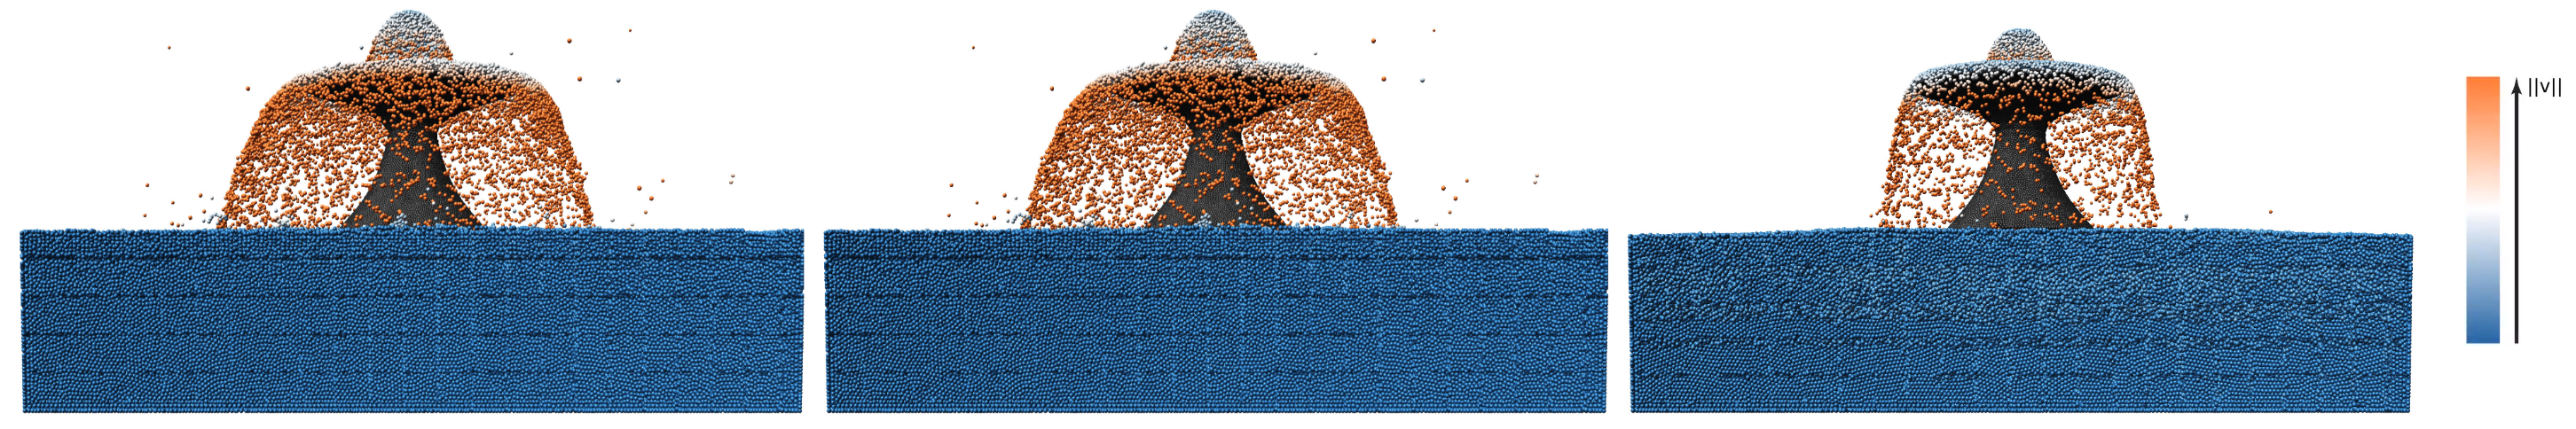
\includegraphics[scale=0.18]{images/9}
	\caption{\label{fig9} Measurements of the magnitude of particle velocities in Fountain scene \cite{reinhardt2017fully}. From left to right are the velocity fields generated by GTS, ITS and ATS respectively. The waterfalls generated by various time stepping models behaves considerably different in terms of overall shape. While in ITS the waterfall leans heavily to the left to form an obviously asymmetric outlook, in ATS the velocity damping causes the particles to travel less distances after they leave the verge of the cone thus forming a steeper waterfall.}
\end{figure}

\subsection{Visual Comparison}
The paper make some visual comparisons on the generated animations to qualitatively analyze the behavior of fluid particles. In particular, it is noticed that ATS dampens the fluid velocities to a small extent where interaction occurs. In the Radial-Flow scene such damping effect may be observed in the disturbed flow regions around the collision object \ref{fig7}. But since an external force field constantly exerts action on the particles, such minor difference fade out soon after the collision. However, in scenarios where no external driving forces occur, such damping leads to visually obvious discrepancies in particle behavior. In the Fountain scenario \ref{fig9}, due to dampened velocities, particles that fall down after collision with the cone form an almost symmetric waterfall that is considerably smaller in size. Additionally, the particles that are propelled upwards at the top of the cone reach only lower heights.
\par
To analyze this effect, the paper computes over time the mean velocity magnitudes of particles in the collision area for both scenes. In the Radial-Flow scenario only particles near the bunny are investigated and in the Fountain test only particles above the pond. The obtained curves are plotted in Fig. \ref{fig10}. Overall, the difference between velocity damping across various time stepping schemes coincide with previous visual inspection. It is worth noting in the Fountain test however, that in ATS the particles only experienced decelerations after initial impact with the cone, implying that proposed asynchronous stepping method does not seem to handle the interactions between fluid particles very well. In this regard, perhaps further improvements on the time integration scheme of the method could be explored.
\par
Apart from the aforementioned flaws, ATS still serves as an equally reliable method to generate visually appealing fluid animation. Especially in regions where heavy interactions occur, the simulation remains stable and the particles travel smoothly even when the largest possible $ \lambda_{v} $ and $ \lambda_{F} $ constants are used.

\begin{figure}[tb]
	\centering
	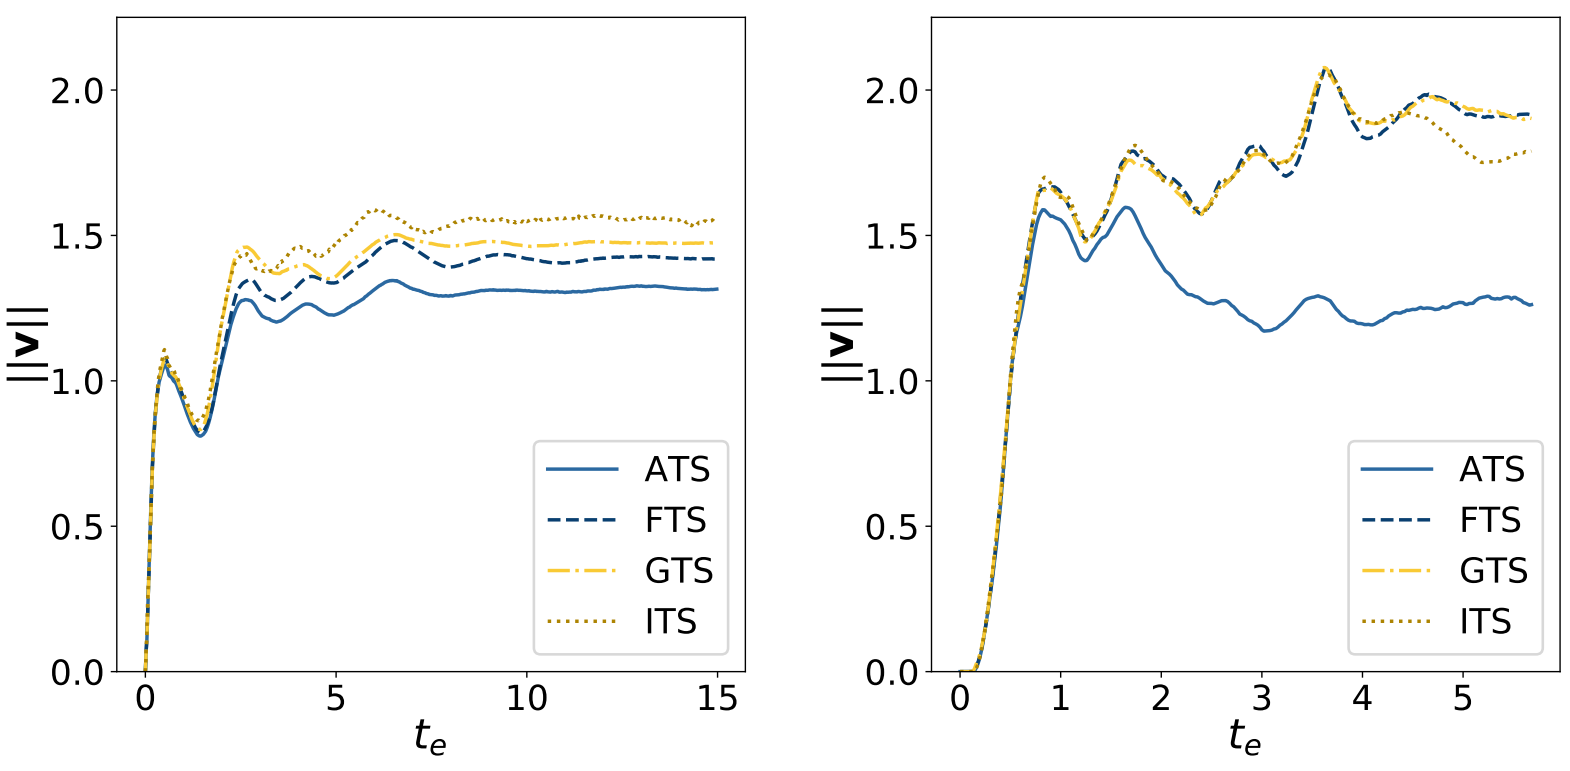
\includegraphics[scale=0.2]{images/10}
	\caption{\label{fig10} Quantitative comparison on the mean velocities of interacting particles in the Radial-Flow scene (left) and Fountain scene (right) \cite{reinhardt2017fully}. In both scenes, ATS demonstrate the most obvious damping effect among all tested methods.}
\end{figure}


\section{Conclusion}

In this paper, the paper presents a novel asynchronous time stepping method for non-iterative SPH integration. Each particle is at each time given a dedicated step size and no global synchronization barriers are introduced to avoid time wasted by waiting threads in previous works. To guarantee local consistency and support attribute computation, neighborhood reconstruction is done each time a particle is processed. A strict chronological processing order of the particles in the form of a priority queue is introduced to enhance stability. A multi-queue-based scheme is smartly devised for parallel execution of this fully asynchronous time integration method. In terms of efficiency, the proposed algorithm is capable of achieving a speedup factor of up to 7.5 and outperforms other tested methods under various scenarios using either serial or parallel execution. In terms of scalability and visual correctness, the respective tests yield some drawbacks of the integration scheme that could be further exploited:

\begin{itemize}
    \item With large proportions of barely moving fluid particles the algorithm's performance boost is undermined. Here the promising work of \cite{goswami2014regional} could be adopted so that the solver handles barely active particles as static ones.
    \item As pointed out by \cite{bender2010boundary}, the acceleration term in Eq. \eqref{eq7} dominates the speed term in non-iterative SPH simulation. A natural idea would be to devise a scheme such that the constants $ \lambda_{v} $ and $ \lambda_{F} $ are automatically adapted for the particles according to their neighborhood information.
    \item Compared to other tested models, asynchronous time stepping leads to higher velocity damping upon interaction with collision objects. Since the paper only implemented a simple boundary handling scheme, in which the particles at domain boundaries are clipped in position, reversed in velocity and applied with a user-defined friction, such damping could be alleviated if a more complex boundary handling model is adopted.
\end{itemize}

\bibliographystyle{alpha}
\bibliography{references}

\end{document}
